\pagestyle{plain}
\graphicspath{{Chapter1/Figs/Raster/}{Chapter1/Figs/}}
\fontdimen2\font=1.2ex
% \chapter{Tổng quan về phát hiện xâm nhập mạng}
\chapter{TỔNG QUAN VỀ PHÁT HIỆN XÂM NHẬP MẠNG}
Trong chương 1, đồ án trình bày cái nhìn tổng quan về các vấn đề về an toàn thông tin mạng, từ đó đưa ra cái nhìn tổng quan đồng thời nêu lên sự cần thiết của bài toán phát hiện xâm nhập mạng, khái niệm của phát hiện xâm nhập mạng. 

Bên cạnh đó, đồ án nêu lên các phương pháp phát hiện xâm nhập mạng đang được nghiên cứu và áp dụng hiện nay và đóng góp của đồ án đã thực hiện được.

\section{Các vấn đề về an toàn thông tin mạng}


\subsection{Mục tiêu của việc đảm bảo an toàn thông tin}
 Với sự phát triển mạnh mẽ của công nghệ thông tin hiện nay, thông tin nắm vai trò cốt lõi, mang tính sống còn đối với các cá nhân, tổ chức, doanh nghiệp và đo đó chúng cũng trở thành mục tiêu hàng đầu của các kẻ tấn công. Thông tin ở đây có thể là thông tin về khách hàng, thông tin về chi tiết kinh doanh hay các thông tin mật. Điểu này đặt ra một vấn đề quan trọng đó chính là phải đảm bảo an toàn thông tin trong suốt quá trình vận hành hệ thống mạng. Đảm bảo an toàn thông tin cho hệ thống mạng là đảm bảo các yếu tố sau:
 \begin{itemize}
     \item Tính xác thực (Authentication): Tính xác thực đảm bảo quá trình truyền tin giữa hai bên đều xác nhận được đối phương mà mình đang giao tiếp. Các phương pháp đảm bảo tính xác thực là : mật khẩu, chữ kí số, vân tay, mống mắt, ...
     \item Tính toàn vẹn (Data Integrity): Tính toàn vẹn dữ liệu đảm bảo quá trình truyền tin giữa hai bên dữ liệu còn nguyên vẹn, không bị sửa đổi, mất mát. Các biện pháp đảm bảo tính toàn vẹn là kiểm soát truy nhập chặt chẽ, xác thực quyền với đối tượng truy nhập dữ liệu, …
     \item Tính bí mật (Confidentiality): Tính bí mật đảm bảo trong quá trình truyền tin, thông tin không bị lộ cho bên thứ ba có thể nghe lén được.
     \item 	Tính sẵn sàng (Availability): Tính sẵn sàng đảm bảo trong quá trình sử dụng, các tài nguyên của hệ thống luôn đáp ứng được nhu cầu của người sử dụng hợp pháp. Các yêu cầu luôn được xử lý kịp thời, không bị gián đonạ
     \item Tính chống chối bỏ (Nonrepudiation): Tính chống chối bỏ ngăn chặn các đối tượng phủ nhận hành vi đã thực hiện đối với hệ thống. Khi một sự cố an toàn thông tin xảy ra thì đây là một yếu tố quan trọng trong quá trình điều tra số.
 \end{itemize}
 
 
\begin{figure}[H]
    \centering
    \smartdiagramset{set color list={orange!60, green!50!lime!60,magenta!60,
blue!50!cyan},
uniform connection color=true,
distance planet-satellite=6cm,
satellite text width=3cm,
planet text width=2.75cm,
}
\smartdiagram[constellation diagram]{Security,  Authentication, Data Integrity, Confidentiality, Availability, Nonrepudiation}
    \caption{Các vấn đề về an toàn thông tin}
     
\end{figure}

\subsection{Tấn công mạng}
Một cuộc tấn công không gian mạng là bất kỳ hình thức tấn công nào của các quốc gia, cá nhân, nhóm hoặc tổ chức nhắm vào các hệ thống thông tin máy tính, cơ sở hạ tầng, mạng máy tính hoặc các thiết bị máy tính cá nhân bằng nhiều cách khác nhau của các hành vi độc hại thường có nguồn gốc từ một nguồn giấu tên, mà đánh cắp, thay đổi, hoặc hủy hoại một mục tiêu cụ thể bằng cách hack vào một hệ thống dễ bị tổn thương.

Các hình thức tấn công mạng tuy ngày càng tinh vi và phức tạp nhưng vẫn có thể chia thành 2 nhóm chính: tấn công bằng phần mềm độc hại và tấn công tài nguyên mạng
\subsubsection*{Tấn công bằng phần mềm độc hại}
Phần mềm độc hại hay còn gọi là Malware là một loại phần mềm hệ thống do các tay tin tặc hay các kẻ nghịch ngợm tạo ra nhằm gây hại cho các máy tính. Tùy theo cách thức mà tin tặc dùng, sự nguy hại của các loại phần mềm ác ý có khác nhau từ chỗ chỉ hiển thị các cửa sổ hù dọa cho đến việc tấn công chiếm máy và lây lan sang các máy khác như là virus trong cơ thể của các sinh vật.
\begin{figure}[H]
    \centering
    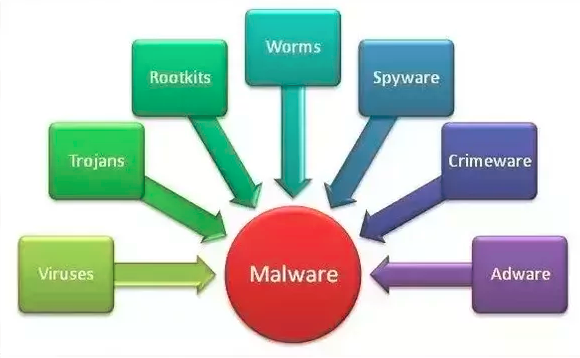
\includegraphics{malware}
    \caption{Malware}
     
\end{figure}
Dưới đây là một vài loại Malware phổ biến hiện nay:
\begin{itemize}
    \item \textbf{Viruses}: Là một chương trình phần mềm có khả năng tự sao chép chính nó từ đối tượng lây nhiễm này sang đối tượng khác (đối tượng có thể là các file chương trình, văn bản, máy tính), thường dùng thực hiện mục đích không tốt. Virus có thể lây vào máy tính qua email, qua các file tải về từ Internet hay copy từ usb và các máy tính khác về… Email là con đường lây lan virus chủ yếu và phổ biến nhất hiện nay. Virus cũng có thể lợi dụng các lỗ hổng phần mềm để xâm nhập từ xa, cài đặt, lây nhiễm lên máy tính một cách âm thầm. Phạm vi phá hoại của virus là rất lớn. Thông thường nhất, các virus thường gây ra mất mát dữ liệu, hư hỏng phần mềm và hư hỏng cả hệ điều hành.
    \item \textbf{Worms}: Có khả năng tự nhân bản trên chính nó mà không cần cấy vào một tập tin lưu trữ. Chúng còn thường sử dụng Internet để lây lan, do đó gây thiệt hại nghiêm trọng cho một mạng lưới về tổng thể, trong khi virus thường chỉ nhắm vào các tập tin trên máy tính bị nhiễm. Worm lây lan chủ yếu là do các lỗ hổng bảo mật của hệ thống. 
    \item \textbf{Trojans}: Là những chương trình hoạt động núp dưới danh nghĩa một phần mềm hữu ích khác, và sẽ thực hiện các khi chương trình giả danh được kích hoạt bởi người sử dụng nhằm đánh cắp thông tin cá nhân, mở các cổng để hacker đột nhập, biến máy tính bị nhiễm thành nguồn phát tán thư rác hoặc trở thành công cụ tấn công một website nào đó. Không như Worm, Trojan horse không có khả năng tự nhân bản để lây lan, cũng như khả năng tự thực thi như virus.
    \item \textbf{Rootkits}: Chủ động “tàng hình” khỏi cặp mắt của người dùng, hệ điều hành và các chương trình anti-virus/anti-malware, rootkit là phần mềm độc hại rất khó bị phát hiện. Rootkit có thể được cài đặt bằng nhiều cách bao gồm việc khai thác lỗ hổng trong hệ điều hành hoặc lấy quyền quản trị máy tính.
    \item \textbf{Spyware}: hay phần mềm gián điệp là thuật ngữ thường được sử dụng để chỉ các phần mềm thực hiện hành vi nhất định như quảng cáo, thu thập thông tin người dùng hoặc thay đổi cấu hình máy tính của người dùng, nói chung là không có sự đồng thuận của người dùng.
    \item \textbf{Crimeware}: Một số nhà cung cấp sử dụng thuật ngữ "crimeware" để chỉ phần mềm độc hại được sử dụng để phạm tội, thường là một tội phạm liên quan đến lợi ích tài chính. Cũng giống như malware, crimeware là một phạm trù rộng gồm hàng loạt các phần mềm độc khác.
    \item \textbf{Adware}: Adware là một loại phần mềm độc hại tải xuống hoặc hiển thị pop-up quảng cáo trên thiết bị của người dùng. Thông thường, Adware không lấy cắp dữ liệu từ hệ thống, nhưng nó buộc người dùng phải xem những quảng cáo mà họ không muốn trên hệ thống. Một số hình thức quảng cáo cực kì gây khó chịu cho người dùng đó là tạo ra pop-up trên trình duyệt mà không thể đóng lại được. Đôi khi người dùng tự lây nhiễm adware được cài đặt mặc định khi tải về những ứng dụng khác mà không hề hay biết.
\end{itemize}
\subsubsection*{Tấn công tài nguyên mạng}

Quá trình truyền và gửi thông tin giữa 2 thực thể trong mạng có thể gặp các kiểu tấn công sau:
\begin{figure}[H]
    \centering
    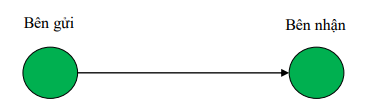
\includegraphics{normal-traffic}
    \caption{Luồng dữ liệu bình thường}
     
\end{figure}
\begin{itemize}
    \item \textbf{Tấn công gián đoạn (Interuption)}: Đây là phương pháp tấn công phá vỡ tính sẵn sàng của hệ thống. Khi bị tấn công gián đoạn, việc truyền tin giữa 2 thực thể trong mạng sẽ gặp khó khăn. Cách tấn công này đôi khi còn gọi là tấn công từ chối dịch vụ (Denial of Services - DoS). Một vài cách tấn công phổ biến là: SYN flood, Smurf, Ping of Death,...
    \begin{figure}[H]
        \centering
        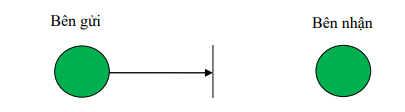
\includegraphics{interuption}
        \caption{Tấn công gián đoạn}
         
    \end{figure}
    \item \textbf{Tấn công nghe trộm (Interception)}: Kiểu tấn công này nhằm mục đích phá hủy tính bí mật của hệ thống. Thông tin được truyền đi giữa 2 thực thể trong mạng bị bên thứ ba nghe lén và thu thập. Một số phương pháp phổ biến dạng này là: Scan port, Packet sniffer,...
    \begin{figure}[H]
        \centering
        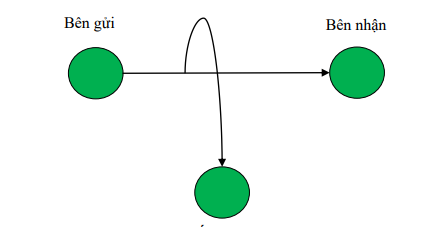
\includegraphics{interception}
        \caption{Tấn công nghe trộm}
         
    \end{figure}
    \item \textbf{Tấn công sửa đổi (Modification)}: Đây là kiểu tấn công nhằm phá vỡ tính toàn vẹn của hệ thống. Dữ liệu trên kênh truyền sẽ bị sửa đổi so với ban đầu khiến cho thông tin bên nhận có được sẽ bị sai lệch so với khi gửi đi.
    \begin{figure}[H]
        \centering
        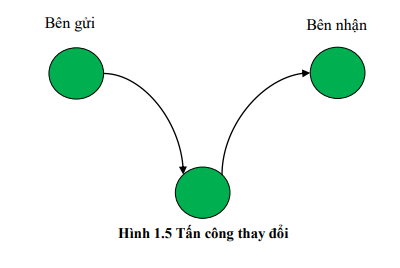
\includegraphics{modification}
        \caption{Tấn công sửa đổi}
         
    \end{figure}
    \item \textbf{Tấn công giả mạo (Fabrication)}: Kiểu này tấn công vào tính xác thực của hệ thống. Kẻ tấn công sẽ tìm cách mạo danh để gửi các thông điệp độc hại hoặc vượt qua các khâu xác thực. 
    \begin{figure}[H]
        \centering
        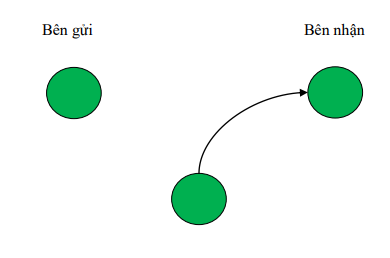
\includegraphics{fabrication}
        \caption{Tấn công giả mạo}
         
    \end{figure}
\end{itemize}
\subsection{Các biện pháp phòng chống tấn công, xâm nhập mạng}
\subsubsection*{Chiến lược an toàn hệ thống}
Các hệ thống mạng không nên sử dụng một phương pháp an toàn duy nhất mà nên có nhiều cơ chế án toàn khác nhau để chúng hỗ trợ lẫn nhau và có thể đảm bảo an toàn ở mức cao.

\begin{figure}[H]
    \centering
    \smartdiagramset{set color list={orange!60, green!50!lime!60,magenta!60,
blue!50!cyan},
uniform connection color=true,
distance planet-satellite=6cm,
satellite text width=3cm,
planet text width=2.75cm,
}
\smartdiagram[constellation diagram]{Least Privilege,  Defense in Depth, Weakest Link, Fail-Safe Stance, Diversity of Defense, Simplicity, Choke Point}
    \caption{Các chiến lược an toàn hệ thống}
     
\end{figure}
\begin{itemize}
    \item \textbf{Quyền tối thiểu (Least Privilege)}: Đây là nguyên tắc cơ bản nhất của an toàn thông tin. Quyền tối thiểu có nghĩa là bất kỳ đối tượng nào (người dùng, quản trị viên, chương trình, hệ thống, hoặc bất cứ điều gì) chỉ nên có các đặc quyền mà đối tượng cần thực hiện nhiệm vụ được giao - không được nhiều hơn. Quyền tối thiểu là một nguyên tắc quan trọng để hạn chế các cuộc tấn công và thiệt hại gây ra từ các cuộc tấn công đó.
    \item \textbf{Phòng thủ theo chiều sâu (Defense in Depth)}: Không phụ thuộc vào một cơ chế an toàn duy nhất, dù mạnh; thay vào đó, cài đặt nhiều cơ chế hỗ trợ nhau. 
    \item \textbf{Điểm thắt (Choke Point)}: buộc các kẻ tấn công sử dụng một kênh hẹp, mà quản trị viên có thể giám sát và kiểm soát. Có thể có nhiều ví dụ về những điểm thắt trong thực tế: trạm thu phí trên cầu, máy an ninh tại siêu thị, quầy bán vé tại rạp chiếu phim.
    \item \textbf{Liên kết yếu nhất (Weakest Link)}: Chiến lược này dựa trên nguyên tắc: " Một dây xích chỉ chắc tại mắt duy nhất, một bức tường chỉcứng tại điểm yếu nhất". 
    
    Kẻ phá hoại thường tìm những chỗyếu nhất của hệ thống để tấn công, do đó ta cần phải gia cố các yếu điểm của hệ thống. Thông thường chúng ta chỉ quan tâm đến kẻ tấn công trên mạng hơn là kẻ tiếp cận hệ thống, do đó an toàn vật lý được coi là yếu điểm nhất trong hệ thống.
    \item \textbf{Lập trường thất bại an toàn(Fail-Safe Stance)}: Trong phạm vi có thể, hệ thống nên có cơ chế thất bại an toàn. Có nghĩa là khi hệ thống bị sụp đổ, nó sẽ từ chối truy cập từ người dùng bất hợp pháp và cả người dùng hợp pháp cho đến khi lỗi được khắc phục. Đây là một hình thức đánh đổi chấp nhận được. 
    \item \textbf{Phòng thủ đa dạng (Diversity of Defense)}: Hơi giống so với phòng thủ theo chiều sâu, nhưng phòng thủ đa dạng có một chút khác biệt. Đó là hệ thống không những cần được phòng thủ nhiều tầng mà mỗi tầng lại phải có nhiều phương pháp phòng thủ khác nhau. 
    \item \textbf{Đơn giản hóa (Simplicity)}: Hệ thống phải được đơn giản hóa. Điều này xuất phát từ 2 lý do. Thứ nhất, hệ thống càng đơn giản thì càng dễ hiểu. Sẽ không đánh giá được một hệ thống có an toàn hay không nếu không hiểu rõ về nó. Thứ hai, các chương trình càng phức tạp thì nguy cơ lỗi càng cao hơn. Đây là một vấn đề lớn trong an toàn thông tin.
\end{itemize}

\subsubsection*{Các biện pháp ngăn chặn xâm nhập}
Không thể có một giải pháp an toàn tuyệt đối nên người ta thường phải sử dụng đồng thời nhiều mức bảo vệ khác nhau tạo thành nhiều hàng rào chắn đối với các hoạt động xâm nhập. Việc bảo vệ thông tin trên mạng chủyếu là bảo vệ thông tin cất giữ trong máy tính, đặc biệt là các máy chủ trên mạng. Bởi thế ngoài một số biện pháp nhằm chống thất thoát thông tin trên đường truyền mọi cố gắng tập trung vào việc xây dựng các mức rào chắn từ ngoài vào trong cho các hệ thống kết nối vào mạng. 
\begin{itemize}
    \item \textbf{Tường lửa}: Tường lửa được xem như một công cụ dùng để hạn chế truy cập vật lý tới máy tính. Chỉ có các thông điệp từ các host đã được xác thực mới được truyền qua tường lửa.
    \item \textbf{Bảo vệ vật lý}:  Ngăn cản các truy nhập vật lý vào hệ thống. Thường dùng các biện pháp truyền thống như ngăn cấm tuyệt đối người không phận sự vào phòng đặt máy tính, dùng ổ khoá trên máy tính hoặc các máy trạm không có ổ đĩa...  
    \item \textbf{Mã hóa dữ liệu}: Mã hóa có nhiệm vụ chuyển các thông điệp sang dạng không thể đọc được trước khi truyền đi. Trong quá trình truyền tải trong mạng, thông điệp luôn ở dạng không thể đọc được và chỉ có bên nhận mới có thể giải mã thông điệp đó.
    \item \textbf{Xác thực}: Mỗi người sử dụng muốn được tham gia vào mạng để sử dụng tài nguyên
đều phải được đăng ký tên và mật khẩu trước.
    \item \textbf{Phân quyền truy nhập}: Lớp bảo vệ trong cùng nhằm kiểm soát các tài nguyên của mạng và quyền hạn trên tài nguyên đó. Dĩ nhiên là kiểm soát được các cấu trúc dữ liệu càng chi tiết càng tốt. Hiện tại việc kiểm soát thường ở mức file. Tùy vào từng người dùng cụ thể mà có những quyền khác nhau: đọc, ghi, sửa xóa file.
    \item \textbf{Hệ thống phát hiện xâm nhập mạng}: Phát hiện xâm nhiệp là quá trình theo dõi các sự kiện xảy ra trên hệ thống máy tính hay hệ thống mạng, phân tích chúng để tìm ra các dấu hiệu xâm nhập bất hợp pháp. Xâm nhập bất hợp pháp được định nghĩa là sự cố gắng tìm mọi cách để xâm hại đến tính toàn vẹn, tính sẵn sàng,... hoặc việc vượt qua các cơ chế bảo mật của hệ thống máy tính hoặc mạng đó. Việc xâm nhập có thể xuất phát từ một kẻ tấn công trên mạng Internet hoặc cũng có thể từ người dùng được phép trong hệ thống muốn chiếm thêm các quyền.
\end{itemize}
\section{Sự cần thiết của phát hiện xâm nhập mạng}

\indent Bình thường, các máy tính chạy ở chế độ cho phép mở nhiều dịch vụ cùng lúc trên cùng một host. Những dịch vụ này cho phép kết nối giữa các host trong mạng với nhiều dạng kiến trúc, hệ điều hành cũng như các chức năng như FTPServer, Webserver,.... Điều này sẽ khiến hệ thống luôn tiềm ẩn các nguy cơ, lỗ hổng có thể khai thác như người dùng không được xác thực có thể truy cập vào hệ thống, ăn cắp các thông tin hoặc thực thi các hành vi động hại. Đây là điều không mong muốn và cần được ngăn ngừa.\\
\indent Như đã trình bày ở trên, tường lửa và mã hóa có thể ngăn ngừa việc khai thác. 2 kỹ thuật trên chỉ nâng cao khả năng bảo mật trong mạng nhưng nó không phải phương pháp có thể giải quyết tất cả mọi vấn đề. Một vài dịch vụ như HTTP service hay SMTP service luôn mở công khai (tường lửa cho phép mọi gói tin đi qua). Các yêu cầu nghiêm ngặt về thời gian thực thi cho các dịch vụ công khai thông dụng không phù hợp với việc sử dụng mã hóa, vì chúng làm cho việc truyền tải các thông điệp chậm hơn. Do đó, những dịch vụ kiểu này là mục tiêu phổ biến để tấn công.

Trong thực tế, các hệ thống thường có các dịch vụ chạy công khai ra ngoài như DNS Server, Mail Server, Webserver, ... Những dịch vụ như này sẽ phải đối mặt với các mối đe dọa đến từ hacker, những kẻ luôn muốn chiếm quyền truy cập trái phép vào hệ thống.  \\

\indent Giả sử với hệ thống mạng của một bệnh viện như sau: 
Bệnh viện muốn cung cấp thông tin của mình tới khách hàng qua Webserver www và cho phép người dùng gửi mail qua hệ thống Mail server. Hệ thống mạng của bệnh viện được bảo vệ bởi tường lửa, đảm bảo việc các kết nối từ Internet công cộng đều chỉ truy cập được vào mail, www và dns.\\

\begin{figure}[H]
    \centering
    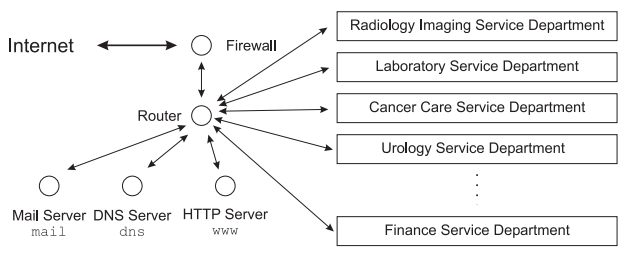
\includegraphics{hospital}
    \caption{Hệ thống mạng bệnh viện}
\end{figure}{}

\indent Hacker luôn muốn các cuộc tấn công phải được xuất phát từ nơi mà danh tính thực của chúng được che giấu, vì vậy hệ thống của công ty này là mục tiêu tốt đối với chúng. Trước khi có thể xâm nhập vào hệ thống, hacker thường thu thập các thông tin công khai có thể hữu ích cho việc tấn công nhiều nhất có thể. Do đó, kẻ tấn công thường sử dụng các nguồn công khai. Trong trường hợp của người viết luận, kẻ tấn công sử dụng các công cụ như nslookup, nmap để tìm các cổng và dịch vụ trong hệ thống. Bên cạnh đó, kẻ tấn công sẽ cố gắng thu thập các thêm các thông tin phụ như các dịch vụ đã biết ở trong các host (dns, mail, www) và thông tin liên lạc của quản trị viên. Giả sử hacker tìm được phiên bản của mail server, sau đó hacker sẽ tìm kiếm trên Internet các nguy cơ bảo mật của phiên bản này. Một lỗ hổng cho phép khai thác lỗ hổng tràn bộ đệm (buffer overflow) được tìm ra. Hacker thực hiện việc khai thác, chiếm quyền quản trị viên khi sử dụng command shell, giúp hacker có thể cài vào đó một backdoor. Với backdoor này, hacker có thể chèn mã độc, đánh cắp thông tin hoặc sử dụng các tài nguyên hệ thống vào các mục đích khác. Trong trường hợp này, tường lửa không giúp bảo vệ hệ thống khỏi kẻ tấn công ở bên ngoài mạng.\\
\indent Ví dụ trên cho thấy các phương pháp bảo mật truyền thống không thể giúp ngăn ngừa hệ thống khỏi các cuộc tấn công từ bên ngoài. Điều này thậm chí có thể đe dọa đến cuộc sống khi hacker có thể thay đổi hệ thống đèn giao thông, gây ra chết người. 
Hệ thống phát hiện xâm nhập mạng là một phương pháp bổ sung cho các khuyết điểm của các phương pháp bảo mật truyền thống. Các hệ thống này tìm cách phát hiện ra các sự cố, xâm nhập bằng cách phân tích các thông tin có thể thu thập được. Trái với phương pháp bảo mật một lớp đã giới thiệu trên, IDS là một phần của phương pháp Bảo mật theo chiều sâu (Defense -in-depth). Trong cách tiếp cận này, một loạt các kỹ thuật (với nhiều mức độ khác nhau) được sử dụng, khi một kỹ thuật thất bại, một kỹ thuật khác sẽ được sử dụng để ngăn cản cuộc tấn công. Bộ cảm biến (sensor) của IDS sẽ phân tích các dữ liệu thu thập được và xác định xem liệu có một cuộc tấn công diễn ra hay không. \\

\indent Thậm chí khi kẻ tấn công có thể xâm nhập vào mạng, các hành động sau đó của hắn có thể được phát hiện với IDS. Việc quét cổng (scan port) của kẻ tấn công với mục đích tìm ra các host và port chứa lỗ hổng có thể bị phát hiện bởi các network-based IDS chỉ trong vài giây. Ngay ca khi kể tấn công có thể thực thi các phầm mềm bắt các gói tin với hi vọng tìm được account/password của nạn nhân thì việc này cũng có thể được cảnh báo. 
Rất nhiều loại cảnh báo khác nhau sinh ra bởi IDS được sử dụng để chống lại việc xâm nhập ngay từ những bước đầu tiên, người quản trị sẽ nhận được thông báo qua e-mail, SMS hoặc tương tự. Khi việc xâm nhập bị phát hiện, attacker có thể bị log out hoặc các tài khoản bị xâm nhập có thể được tắt ngay lập tức, các file quan trọng được khôi phục từ một hệ thống backup, các tiến trình không xác định sẽ được đóng lại. Tường lửa sẽ được tự động cấu hình lại, chỉ kết nối từ một số nguồn tin cậy. Hệ thống sẽ được chuyển về trạng thái an toàn khi người quản trị được cảnh báo kịp thời.\\

% Hệ thống phát hiện xâm nhập là một phương án tốt để phát triển tính an toàn của hệ thống. Thật không may, các hacker cũng có thể xâm nhập vào các IDS và phân tích cách hoạt động của IDS. Các hacker có thể tìm ra các hành động nào sẽ bị hệ thống phân loại là xâm nhập cũng như các điểm yếu của hệ thống. 

\section{Phân loại phát hiện xâm nhập}
\subsection{Phân loại theo kỹ thuật phát hiện}

Việc phát hiện xâm nhập được tiến hành nhờ vào quá trình giám sát các sự kiện xảy ra trong hệ thống máy tính hay mạng và phân tích xem có dấu hiệu của việc xâm nhậ  hay không. Hệ thống phát hiện xâm nhập (IDS) có thể là hệ thống phần cứng hay phần mềm cho phép tự động hóa quá trình phát hiện hành vi xâm nhập. 

Về cơ bản có ba phương pháp chính dựa theo các dấu hiệu/chữ ký; bất thường; và đặc tả, còn gọi là phân tích giao thức có trạng thái (stateful protocol analysis). 

Các dấu hiệu thường là các mô hình hay chuỗi ký tự tương ứng với các vụ tấn công hay mối đe dọa đã biết. Để phát hiện IDS so sánh các mô hình với các sự kiện thu được để nhận biết việc xâm nhập. Phương pháp này còn được gọi là phương pháp dựa trên tri thức do sử dụng cơ sở tri thức về các hành vi xâm nhập trước đó. 

Với phương pháp dựa trên bất thường thì sự bất thường được coi là sự khác biệt với hành vi đã biết bằng các lập hồ sơ các hành vi thông thường lập từ việc theo dõi các hoạt động thường xuyên, kết nối mạng, máy trạm hay người dùng qua một khoảng thời gian. Hệ thống phát hiện so sánh các hồ sơ với các sự kiện quan sát được để nhận biết các vụ tấn công nghiêm trọng 

IDS phát hiện theo đặc tả nhận biết và theo dõi được trạng thái các giao thức (sự tương ứng giữa cặp yêu cầu/đáp ứng). Việc xây dựng đặc tả phụ thuộc vào nhà cung cấp giao thức.

Phần dưới đây giới thiệu hệ thống phân loại theo \cite{9} bao gồm 5 cách tiếp cận chính
như sau:

\begin{itemize}
    \item Thống kê chủ yếu dựa trên thiết lập ngưỡng, giá trị trung bình, phương sai, và
xác suất để xác định hành vi xâm nhập. Phương pháp này dựa trên độ đo
khoảng cách, công thức Bayes, lý thuyết trò chơi \cite{11} sử dụng nguồn dữ liệu từ
hồ sơ người dùng, dữ liệu kiểm toán hay viêc sử dụng tài nguyên máy tính như
bộ nhớ và bộ xử lý.
    \item Đối sánh mẫu chủ yếu dùng để phát hiện xâm nhập đã biết bằng cách đối sánh
mẫu, giám sát bàn phím, mạng Petri như giới thiệu trong \cite{12}. Nguồn dữ liệu sử
dụng ngoài các dữ liệu kiểm toán cần thêm hồ sơ người dùng, bản ghi phím
bấm và các mẫu luật từ hồ sơ người dùng và chính sách sử dụng.
    \item Luật bằng cách thuật toán dựa trên véc-tơ học máy SVM, khai phá dữ liệu như
trong \cite{2}. Phương pháp này cho phép tự động xây dựng và cập nhật mô hình
phát hiện giúp cho hệ thống được linh hoạt và mềm dẻo hơn.
    \item Trạng thái dựa trên việc phân tích trạng thái bằng mô hình Markov, phân tích
giao thức như trong \cite{9}.
    \item Kinh nghiệm sử dụng mạng nơ-ron, lô-gíc mờ, thuật toán gen như \cite{13,14}.
Phương pháp này có thể sử dụng dữ liệu từ lưu lượng mạng, thông tin từ các
vụ việc xâm nhập thành công trước đó.
\end{itemize}

\subsection{Phân loại theo công nghệ}

Xét về khía cạnh công nghệ để xây dựng và triển khai các hệ thống ngăn ngừa
xâm có thể phân thành 4 loại cơ bản như dưới đây.
\subsubsection*{Phát hiện xâm nhập cho máy trạm HIDS}

Mục tiêu của hệ thống này là giám sát và thu thập các đặc trưng về các máy
trạm (host) chứa đựng các thông tin nhạy cảm, máy chủ và các hoạt động đáng
ngờ.

Hệ thống có thể triển khai trên mạng thông thường hoặc có quản lý (an toàn) và thực hiện việc thu thập thông tin về các hoạt động của ứng dụng và lưu lượng mạng.

Hệ thống cung cấp các cảnh báo về các sự cố lớp ứng dụng, lớp vận chuyển và lớp mạng. Tuy nhiên độ chính xác của cảnh báo khó chuẩn xác do thiếu thông tin về ngữ cảnh mà máy tính và chương trình người dùng. Có thể xảy ra việc chậm trễ trong việc cảnh báo và hệ thống kiểu này phải sử dụng tài nguyên của máy trạm để hoạt động được. Trong một số tình huống có thể xung đột với các biện pháp kiểm soát hiện có như các chương trình quét vi-rút hay tường lửa.
\begin{figure}[H]
    \centering
    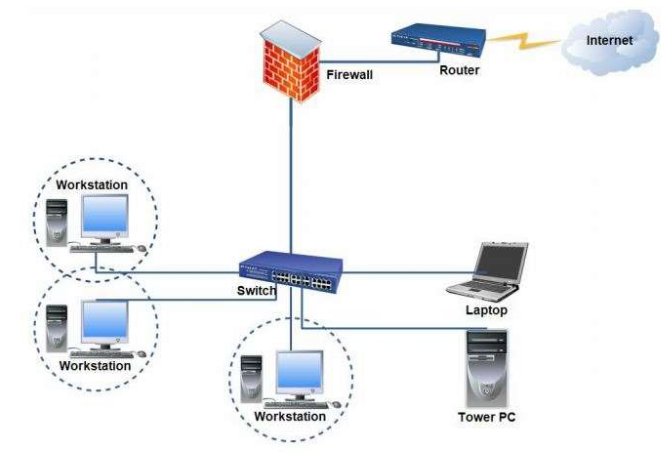
\includegraphics[scale=0.6]{Chapter1/Figs/HIDS.png}
    \caption{HIDS}
     
\end{figure}
\subsubsection*{Phát hiện xâm nhập cho mạng NIDS}

Hệ thống kiểu này thu thập các gói tin tại các phân đoạn mạng nhờ các cảm biến. Sau đó phân tích các hoạt động của ứng dụng và giao thức để phát hiện các hành vi đáng ngờ. Hệ thống thường được triển khai trong mạng có quản lý (an toàn) và thực hiện thu thập thông tin về các trạm, hệ điều hành, ứng dụng, và lưu lượng mạng. Hệ thống có thể cảnh báo việc tấn công, thăm dò lớp ứng dụng, lớp vận chuyển, lớp mạng, các dịch vụ ứng dụng bất thường, xung đột chính sách. Tuy nhiên, hệ thống không giám sát các giao thức mạng không dây WF. Về cơ bản có tỷ lệ nhầm FP-FN cao và không phát hiện được tấn công bên trong lưu lượng được mã hóa. Trong trường hợp hệ thống chịu tải nặng sẽ không thể phân tích đầy đủ.
\begin{figure}[H]
    \centering
    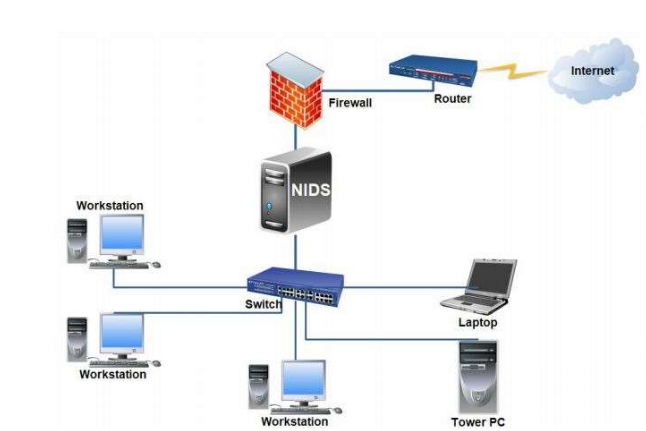
\includegraphics[scale = 0.6]{Chapter1/Figs/NIDS.png}
    \caption{NIDS}
     
\end{figure}

\subsubsection*{Phát hiện xâm nhập cho mạng không dây}
Hệ thống phát hiện có tính năng giống như NIDS song tập trung vào lưu lượng mạng không dây: như mạng ad-hoc, mạng các cảm biến, mạng lưới. Hệ thống này có thể triển khai trên mạng có quản lý hoặc mạng bình thường và thực hiện việc thu thập thông tin về các thiết bị không dây WF. Hệ thống phát hiện thực hiện các cảnh báo các sự cố về các giao thức WF, thiết bị và mạng WF không an toàn, tấn công DOS, quét mạng, xâm phạm chính sách. Tuy nhiên, nhược điểm của hệ thống này là không thể giám sát các hoạt động của giao thức ở lớp trên và không tránh được kỹ thuật lẩn trốn. Mặt khác các cảm biến của hệ thống có thể bị tấn công chèn sóng vật lý và hệ thống không bù trừ được cho các giao thức không an toàn

\subsubsection*{Phát hiện xâm nhập qua phân tích hành vi mạng NBA}

Việc phát hiện xâm nhập qua việc kiểm tra lưu lượng mạng để phát hiện tấn công khi có lưu lượng bất thường. Hệ thống này rất hữu ích trong việc chống thăm dò, dựng lại quá trình lây nhiễm của phần mềm độc hay tấn công DOS và có thể triển khai mạng có quản lý hay mạng bình thường. Hệ thống tiến hành thu thập thông tin về các máy trạm, hệ điều hành, các dịch vụ và đưa ra các cảnh báo các luồng lưu lượng bất thường, các dịch vụ ứng dụng bất thường, quét mạng và vi phạm chính sách \cite{8}.
\subsection{Kết luận}
Mỗi kỹ thuật phát hiện hành vi xâm nhập có điểm mạnh và yếu riêng. Hệ thống dựa trên dấu hiệu hiệu quả với việc phát hiện các tấn công biết trước. Trong khi đó hệ thống dựa trên luật gặp phải vấn đề cập nhật tri thức với các tấn công mới. Hệ thống dựa trên kinh nghiệm gặp khó khăn khi hoạt động ở chế độ thời gian thực do mất nhiều thời gian huấn luyện và đào tạo để hệ thống có khả năng ứng phó với các dạng tấn công mới. Việc có thông tin đầy đủ về các ưu và nhược điểm của mỗi phương pháp giúp lựa chọn, sử dụng hiệu quả các kỹ thuật ngăn ngừa và bố trí một cách phù hợp các hệ thống ngăn ngừa xâm nhập để tăng cường các thuộc tính an toàn của hệ thống.
\section{Mục tiêu của đồ án}
Trên cơ sở tìm hiểu về các kỹ thuật sử dụng trong phát hiện tấn công mạng, đồ án hướng đến xây dựng hệ thống phát hiện tấn công mạng sử dụng phương pháp học có giám sát dựa trên kỹ thuật machine learning mà cụ thể ở đây là thuật toán Boosted Tree . \\
\indent Boosted Tree là một thuật toán học máy khá phổ biến trong việc giải quyết các bài toán phân lớp dữ liệu. Đây là một thuật toán mạnh mẽ, được áp dụng rất nhiều vào các bài toán thực tế. Đồng thời, Boosted Tree cũng là thuật toán được các nhà vô địch các cuộc thi về học máy và khoa học dữ liệu trên trang Kaggle \cite{15}. \\
\indent Đối tượng áp dụng của nghiên cứu trong đồ án là tập dữ liệu UNSW-NB15. Đây là một trong những tập dữ liệu mới nhất dành cho việc nghiên cứu phát hiện xâm nhập mạng. Chi tiết của tập dữ liệu này sẽ được giới thiệu kỹ hơn tại mục 1 chương 3.




